\section{Mechanical analysis}
\subsection{Reference frames}
In order to study the behavior of the robot we will use the following frames:
\begin{itemize}
    \item Absolute frame: From a fix object in the room. 
    \item Body frame: From the body of our robot.
\end{itemize}

\begin{tikzpicture}[]
    \node (left_wheel) [cylinder, shape border rotate=0, draw, minimum height=1mm, minimum width=15mm] {};

    \node (right_wheel) [cylinder, shape border rotate=0, draw, minimum height=1mm, minimum width=15mm] {};

    \coordinate (left_wheel 0 0);
    \coordinate (right_wheel 10 0);



    \end{tikzpicture}


\subsection{Inclination control}
In order to keep the inclination at a certain angle we must be able to compensate all the torque being applied to the body.

Assuming that the body is well balanced and neglecting the torque generated by the friction with air, the sum of all the torques in the motor axis applied to the body is equal to the sum of the torque applied by the motors:

\[\tau_{body} = \sum \tau_{motors}\]

The torque of the motors produce a reaction in the body opposite to the torque that the motors deliver to the wheels and the flywheel.

\[\tau_{body} = -\tau_{right-wheel} -\tau_{left-wheel} -\tau_{flywheel} \]

If we want to control the inclination $\theta$, we must be able to control $\tau_{body}$ in a range $\tau_{body} \in (-\epsilon, \epsilon)$. Observe that the angular acceleration of the body is linearly dependent with the torque it receives. In the limit case $\epsilon = 0$. In order to simplify the calculations we will assume $\epsilon = 0$.

\[0 = -\tau_{right-wheel} -\tau_{left-wheel} -\tau_{flywheel} \Rightarrow \tau_{right-wheel} +\tau_{left-wheel} = -\tau_{flywheel} \]

In other words, we must compensate the torque of the wheels with the torque of the flywheel.

\subsection{Wheels torque}
The wheel torque we can induce is limited by the motor specifications. Note that the maximum torque of the motor is a function of velocity and in particular at max speed the torque is zero.

\[\tau_{motor} (w_{wheel}) \]


We assume that the wheels just roll and do no slip.
The robot is pushed by the wheels that make a force $F_{drag}$ against the ground in the contact point. See figure \ref{fig:Wheel force diagram}.

We can express the torque of the wheel as:
\[ \tau_{wheel} =min(\tau_{motor} (w_{wheel}), I_{wheel} * \dot{w}_{wheel} - F_{drag} * r_{wheel})\]
\begin{figure}[ht]
	\centering
	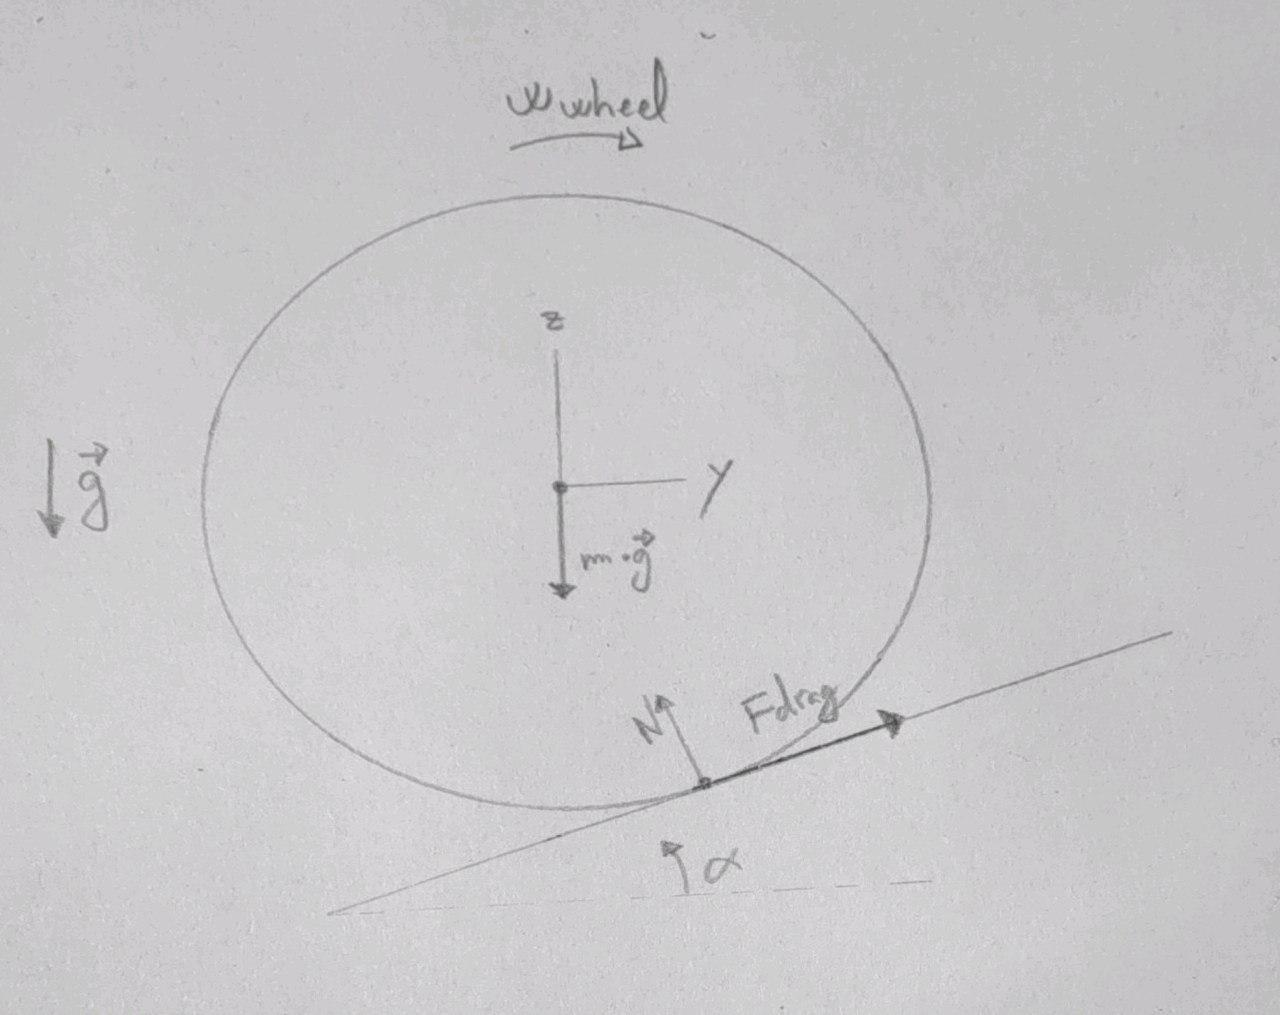
\includegraphics[width=10cm]{img/wheel_diagram.jpg}
	\caption{Wheel force diagram}
	\label{fig:Wheel force diagram}
\end{figure}


\subsection{Flywheel torque}

\begin{figure}
	\centering
	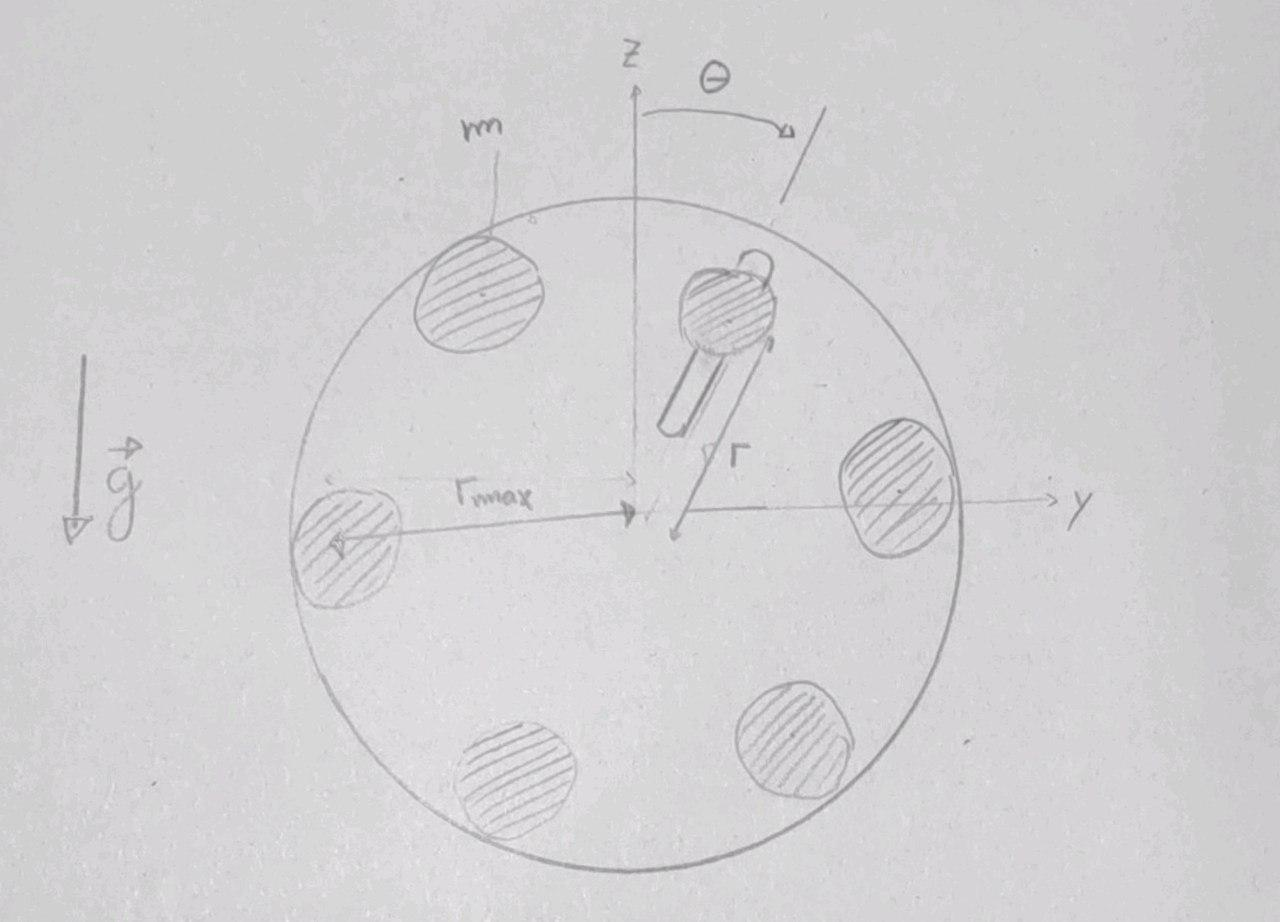
\includegraphics[width=10cm]{img/flywheel_diagram.jpg}
	\caption{Flywheel force diagram}
	\label{fig:Flywheel force diagram}
\end{figure}

The flywheel torque we can induce is also limited by the motor specifications. 

Assuming that a general configuration of the flywheel, see figure \ref{fig:Flywheel force diagram}. we formulate its torque the following way:


\[\tau_{flywheel} = min(\tau_{motor} (w), \ddot{\theta}*I_{flywheel}(r) + m_{cylinder} * g * (r - r_{max}) * \sin{\theta}) \]

\subsection{Motor specifications}

Here we have the factory specifications of our motors: 
\begin{itemize}
    \item Operating voltage: between 3 V and 9 V
    \item Nominal voltage: 6 V
    \item Free-run speed at 6 V: 176 RPM
    \item Free-run current at 6 V: 80 mA
    \item Stall current at 6V: 900 mA
    \item Stall torque at 6V: 5 kg·cm
    \item Gear ratio: 1:35
    \item Reductor size: 21 mm
    \item Weight: 85 g
\end{itemize}

\subsection{Hypothesis}
Assuming that the body is well balanced
